% Created 2026-11-22 Sun 19:27
% Intended LaTeX compiler: pdflatex
\documentclass[aspectratio=169,11pt]{beamer}

\usepackage[utf8]{inputenc}
\usepackage[T1]{fontenc}
\usepackage{graphicx}
\usepackage{longtable}
\usepackage{wrapfig}
\usepackage{rotating}
\usepackage[normalem]{ulem}
\usepackage{amsmath}
\usepackage{amssymb}
\usepackage{capt-of}
\usepackage{hyperref}
\usepackage{booktabs}
\usepackage{tikz}
\usetikzlibrary{positioning}
\usetheme{moloch}
\date{}
\title{Predicción del abandono de clientes en telecomunicaciones}
\subtitle{Lectura crítica de Fujo, Subramanian y Khder (2022)}
\hypersetup{
 pdfauthor={},
 pdftitle={},
 pdfkeywords={},
 pdfsubject={},
 pdfcreator={},
 pdflang={Spanish}}
\begin{document}

\begin{frame}[label={sec:org4c7d978}]{¿Qué clientes van a abandonar?}
\begin{itemize}
\item \emph{Customer churn prediction}: predicción del abandono de clientes.
\item Clasificación binaria: \alert{abandona / no abandona}.
\item Objetivo: orientar acciones de retención hacia clientes en riesgo.
\end{itemize}

\vfill
\footnotesize
\textit{Customer Churn Prediction in Telecommunication Industry Using Deep Learning}.\\
S. W. Fujo, S. Subramanian y M. A. Khder (2022).\\
\textit{Information Sciences Letters}, 11(1), 185--198.\\
\href{https://doi.org/10.18576/isl/110120}{doi:10.18576/isl/110120}
\end{frame}
\begin{frame}[label={sec:orgdbaab05}]{Los datos: clases desequilibradas}
\begin{center}
\begin{tabular}{lrr}
\toprule
Característica & IBM Telco & Cell2Cell\\
\midrule
Clientes & 7.043 & 51.047\\
Variables predictoras & 20 & 57\\
Clientes que abandonan & 26,5 \% & 28,8 \%\\
\bottomrule
\end{tabular}
\end{center}

\begin{itemize}
\item La mayoría de los clientes \alert{no abandona}.
\item Acertar en total no basta: interesa \alert{detectar abandonos} y controlar las \alert{falsas alarmas}.
\end{itemize}

\vfill
\footnotesize Fuente: tabla de características, p. 188.
\end{frame}
\begin{frame}[label={sec:orgeeb8505}]{La propuesta: combinar varias técnicas}
\begin{center}
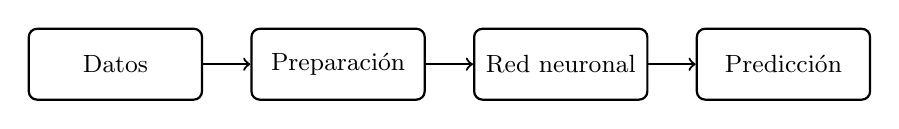
\begin{tikzpicture}[node distance=0.6cm,
  box/.style={rectangle, rounded corners=3pt, draw, thick,
              minimum height=0.9cm, minimum width=2.2cm,
              align=center, font=\small}]
\node[box] (d) {Datos};
\node[box, right=of d] (p) {Preparación};
\node[box, right=of p] (r) {Red neuronal};
\node[box, right=of r] (pr) {Predicción};
\draw[->, thick] (d) -- (p);
\draw[->, thick] (p) -- (r);
\draw[->, thick] (r) -- (pr);
\end{tikzpicture}
\end{center}

\begin{itemize}
\item \alert{Lasso}: selección de variables.
\item \alert{Random Oversampling}: duplicación de ejemplos de la clase minoritaria.
\item \alert{Deep-BP-ANN}: red neuronal entrenada mediante retropropagación.
\item \alert{Regularización de actividad y parada temprana}: control del sobreajuste.
\item Configuración destacada: capas de \alert{250 neuronas}.
\end{itemize}

\vfill
\footnotesize Fuente: método y configuración, pp. 188--190 y 192--195. El esquema resume componentes; no determina cuándo se separan entrenamiento y prueba.
\end{frame}
\begin{frame}[label={sec:org2c7eef6}]{¿Cómo comprueban si funciona?}
\begin{itemize}
\item \alert{Holdout}: 90 \% entrenamiento / 10 \% prueba.
\item \alert{Validación cruzada}: 10 particiones.
\end{itemize}

\begin{center}
\begin{tabular}{ll}
\toprule
Métrica & Pregunta\\
\midrule
Exactitud (\emph{accuracy}) & ¿Cuánto acierta en total?\\
Sensibilidad (\emph{recall}) & ¿Cuántos abandonos detecta?\\
Precisión (\emph{precision}) & ¿Cuántas alertas resultan correctas?\\
\bottomrule
\end{tabular}
\end{center}

\vfill
\footnotesize Fuente: validación y métricas, pp. 190--191.
\end{frame}
\begin{frame}[label={sec:org61566a5}]{Resultados: detección y falsas alarmas}
\small
\begin{center}
\begin{tabular}{llrr}
\toprule
Datos & Evaluación & Exactitud & Sensibilidad \\
\midrule
IBM Telco & Holdout & 88,12\,\% & 93,05\,\% \\
IBM Telco & Validación cruzada & 86,57\,\% & \alert{94,45\,\%} \\
Cell2Cell & Holdout & 79,38\,\% & 89,32\,\% \\
Cell2Cell & Validación cruzada & \alert{73,90\,\%} & 89,74\,\% \\
\bottomrule
\end{tabular}
\end{center}
\normalsize

\begin{itemize}
\item Sensibilidad elevada en ambos conjuntos.
\item Cell2Cell, validación cruzada: precisión del \alert{68,15 \%}.
\item En esa evaluación: unas \alert{32 falsas alarmas por cada 100 alertas}.
\end{itemize}

\vfill
\footnotesize Fuente: tabla de resultados, p. 193. Las cifras corresponden al experimento; su traslado a una población real requiere validación.
\end{frame}
\begin{frame}[label={sec:org5806bd7}]{¿Mejora frente a otras alternativas?}
\begin{itemize}
\item Los autores comunican mejores resultados frente a \alert{XGBoost, regresión logística, Naïve Bayes y KNN}.
\item Comparación con un antecedente: \alert{Cell2Cell, validación cruzada de 10 particiones}.
\end{itemize}

\begin{center}
\begin{tabular}{lr}
\toprule
Modelo & Exactitud\\
\midrule
CNN/LFNN, antecedente & 71,66 \%\\
Deep-BP-ANN, este artículo & 73,90 \%\\
\bottomrule
\end{tabular}
\end{center}

\alert{Diferencia: +2,24 puntos porcentuales.}

\begin{alertblock}{Cautela}
Mismo conjunto de datos no garantiza idénticas condiciones experimentales.
\end{alertblock}

\vfill
\footnotesize Fuentes: comparación interna, pp. 192--193; antecedente de Umayaparvathi e Iyakutti (2017), recogido en p. 194.
\end{frame}
\begin{frame}[label={sec:org1de7dfa}]{Limitaciones de la evaluación}
\begin{enumerate}
\item \alert{Posible fuga de datos.}
No se aclara el orden entre sobremuestreo y partición. Si se duplica antes de dividir, podría haber copias en entrenamiento y prueba.
\item \alert{Entrenamiento diferente entre protocolos.}
Parada temprana en holdout; número fijo de épocas en validación cruzada.
\item \alert{Reproducibilidad e incertidumbre.}
Faltan detalles de configuración y medidas de variación de los resultados.
\end{enumerate}

\alert{La fuga de datos es un riesgo, no un error demostrado.}

\vfill
\footnotesize Valoración crítica de la descripción del método y la evaluación, pp. 188--190 y 192--195.
\end{frame}
\begin{frame}[label={sec:orgc54a0ec}]{Conclusión}
\begin{itemize}
\item \alert{Propuesta}: combinar una red neuronal con selección de variables, equilibrado y control del sobreajuste.
\item \alert{Resultado}: alta sensibilidad en los experimentos presentados.
\item \alert{Pendiente}: evaluación más transparente, reproducible y comparable.
\end{itemize}

\bigskip
\begin{block}{Idea final}
Resultados prometedores, pero evidencia insuficiente para afirmar una superioridad definitiva en una aplicación real.
\end{block}
\medskip
\centering\textit{¿Qué haría falta para confiar en este modelo en producción?}
\end{frame}
\end{document}
